\chapter{Minimalflächen\label{chapter:minimal}}
\lhead{Minimalflächen}
\begin{refsection}
\chapterauthor{Nadja Rutz und Ambroise Suter}

\section{Einleitung}
 \label{A_Einleitung}
\rhead{Einleitung}
Was sind Minimalflächen? 
Wie werden sie definiert? 
Warum passen sie in den Kontext dieses Buches?
Diese Fragestellungen werden im Laufe dieses Kapitel an Hand von Beispielen illustriert und erörtert.

Wie der Name erahnen lässt, beschreiben Minimalflächen Flächen mit minimalem Flächeninhalt. 
Ein gängiges Beispiel aus der Physik sind Seifenfilme. Wenn die Luft auf beiden Seiten eines Seifenfilms den gleichen Druck hat, dann ist er eine Minimalfläche.


\section{Katenoid}
 \label{A_Katenoid}
\rhead{Katenoid}
Wenn man zwei koaxiale Drahtringe parallel zueinander in Seifenwasser taucht, entsteht eine Rotationsfläche, (Abbildung \ref{KatenoidSeifenfilm}) welche Katenoid genannt wird. 

Das Katenoid ist die erste entdeckte Minimalfläche.
Sie wurde schon 1776 von Jean Baptiste Meusnier erstmals beschrieben.
In diesem Abschnitt wird die Funktion des Katenoids mit Hilfe der Eulerschen Differentialgleichung, der Variationsrechnung hergeleitet.
\subsubsection{Beispiel Katenoid als Rotationsfläche}

\begin{figure}
  \centering
  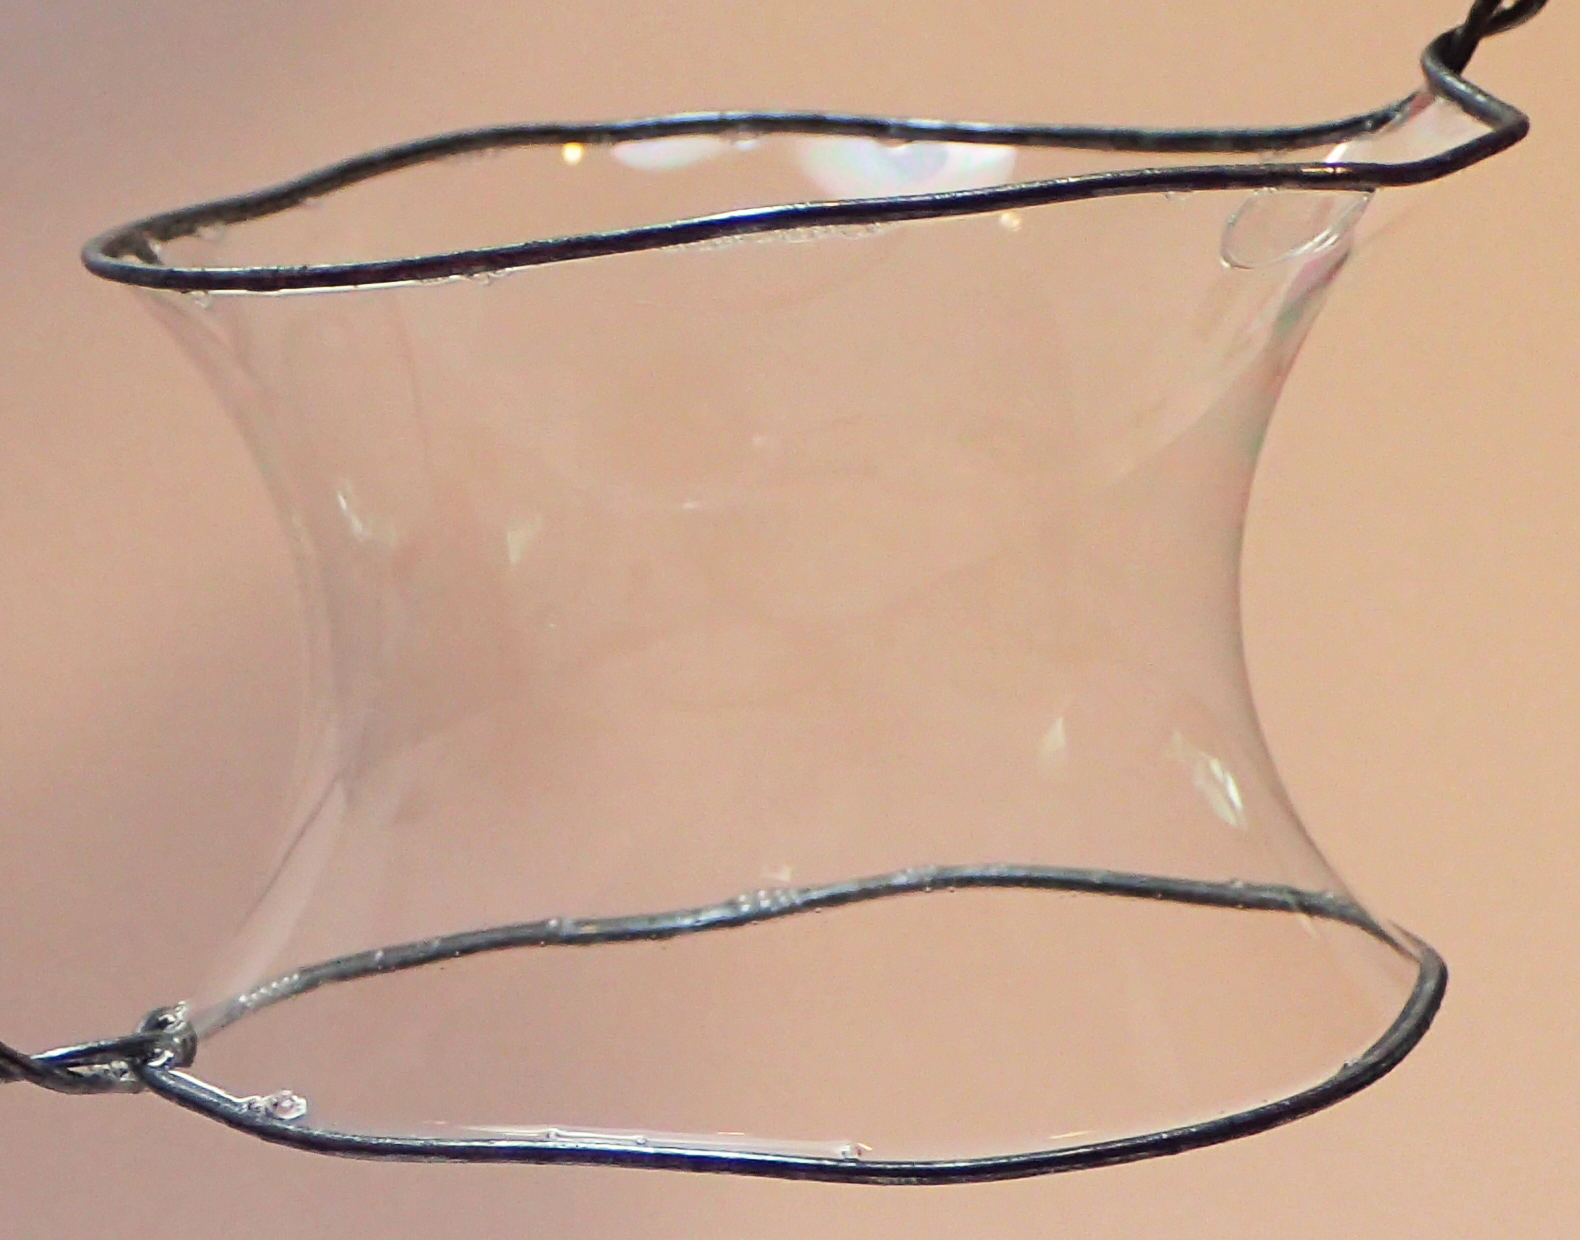
\includegraphics[scale=0.5]{minimal/Cartenoid_Foto.png}
  \caption{Seifenfilm Katenoid} 
  \label{KatenoidSeifenfilm}
\end{figure}


\begin{figure}
  \centering
  \includegraphics[scale=0.3]{minimal/Catenoid34Black.pdf}
  \caption{Skizze Katenoid} 
  \label{Katenoid}
\end{figure}
In der Skizze \ref{Katenoid} ist ein Katenoid abgebildet, bei welchem in Bezug auf die $z$ Achse der untere Drahtring bei $-L$ und der obere bei $+L$ ist. 
Die beiden Kreise sollen die gleichen Radien haben, also gilt $r(-L)=r(+L)=R$. 
Die Flächenpunkte des Katenoids werden mit der Funktion $r(z)$ beschrieben. Diese wird um die Rotationsachse $z$ rotiert, um den Flächeninhalt des Katenoids zu berechnen.
Hierzu braucht man eine Gleichung, welche eine Länge entlang eines Meridians auf der Katenoidoberfläche beschreibt. 
Mit Hilfe des Satzes von Pythagoras (Abbildung \ref{Katenoid}) kann man $ds^2=dz^2+dr^2$ schreiben.
Formt man diese Gleichung um nach $ds$, erhält man die Gleichung

\begin{equation} \label{ds}
  ds=\sqrt{dz^2\bigg(1+\frac{dr^2}{dz^2}\bigg)}= \sqrt{dz^2(1+\dot r^2)}=\sqrt{(1+\dot r^2)}\,dz .
\end{equation}
\subsubsection{Minimalflächeneigeschaft}
Der Seifenfilm bewegt sich automatisch in den minimalenergetischen Zustand. 
In diesem Zustand ist dann auch der Flächeninhalt $S$ des Seifenfilms minimal.
Demzufolge muss das Integral 
\begin{equation} \label{S1}  
  S= \int 2 \pi r \,ds 
\end{equation}
minimiert werden. 
Durch Einsetzen von Gleichung \eqref{ds} erhält man die Gleichung 
\begin{equation} \label{S2}
  S=2 \pi \int_{-L}^{+L} r\sqrt{1+\dot r^2}\,dz =2 \pi \int_{-L}^{+L}  F(r,\dot r, z) \,dz  ,
\end{equation}
welche man als Funktion 
\begin{equation} \label{F}
 F(r,\dot r, z) = r \sqrt{1+\dot r^2}
\end{equation}
noch etwas übersichtlicher schreiben kann.



Um dieses Integral \eqref{S2} zu minimieren kann man sich der Eulerschen Differentialgleichung der Variationsrechnung bedienen. 
\subsubsection{Variationsrechnung}
Die Eulersche Differentialgleichung der Variationsrechnung wird im Kapitel \ref{skript:geodaeten:section:variationsprinzip}  der Geodäten genauer erklärt.
Das Anwendungsprinzip wird hier kurz zusammengefasst. Hat man ein Integral $I$, welches von einer Funktion $y(x)$ abhängt, kann man die Eulersche Differentialgleichung anwenden, um die Funktion $y(x)$ zu finden, für welche das Integral $I$ extrem wird. Die Eulersche Differentialgleichung besagt, dass anstelle des Ausrechnens  einer Integralfunktion der Art \begin{equation} \label{E_DGL1}  
  I(y)= \int_a^b F(x,y(x),\dot y(x))\,dx ,       
\end{equation}
auch die Differentialgleichung  



\begin{equation} \label{E_DGL2}
\bigg(\frac{\partial F}{\partial y}\bigg)- \frac{d}{dx} \bigg(\frac{\partial F}{\partial \dot{y}}\bigg)=0         
\end{equation}
gelöst werden kann.

Die Gleichung \eqref{S2} für den Flächeninhalte des Katenoids ist ein solches Integral, da es von der Funktion $r(z)$ abhängt und die Aufgabe ist es eben diese zu finden. Wendet man also das Prinzip der Variationsrechnung an, erhält man die Differentialgleichung
\begin{equation} \label{K_DGL1}
\bigg(\frac{\partial F}{\partial r}\bigg)- \frac{d}{dz} \bigg(\frac{\partial F}{\partial \dot{r}}\bigg)=0 .
\end{equation}
Setzt man $F$ aus der Gleichung \eqref{F} ein, erhält man
\begin{equation} \label{K_DGL_H}
\sqrt{1+{\dot {r}}^2}-\frac{ d }{ dz } \bigg( r \frac{ 1 }{2  }\left( {1+{\dot {r}}^2}  \right)^{-1/2} 2 \dot {r}\bigg)=0 .
\\
\end{equation}
Dies wird nun schrittweise umgeformt, zunächst durch Ausrechnen der Ableitung
\begin{equation} \label{K_DGL_H2}
\left(1+{\dot {r}}^2  \right)^{-1/2}-\bigg(r \frac{ -1 }{2  } \left({1+{\dot {r}}^2}  \right)^{-3/2} 2 \dot{r} \ddot{r}  \dot{r}+ r \left({1+{\dot {r}}^2}  \right)^{-1/2} \ddot{r} +\dot{r} \left({1+{\dot {r}}^2}  \right)^{-1/2} \dot{r}\bigg)=0
\end{equation}
bis die Differentialgleichung zweiter Ordnung  
\begin{equation} \label{K_DGL_R}
1+{\dot {r}}^2=r  \ddot{r}
\end{equation}
entsteht. 
Gesucht ist also eine Funktion $r(z)$, die die Differentialgleichung \eqref{K_DGL_R} erfüllt. Als Randbedingungen für die Funktion $r(z)$ sind in diesem Beispiel $r(+L)=R$ und $r(-L)=R$ aus der Abbildung \ref{Katenoid} gegeben.

\subsubsection{Lösen der Differentialgleichung}
Die Differentialgleichung zweiter Ordnung \eqref{K_DGL_R} kann mit Hilfe einiger mathematischer Umformungen, Aufleiten und hyperbolischer Trigonometrie gelöst werden. 
Dies ist eine langwierige Berechnung und wird daher hier nicht durchgeführt.

Anstelle des konkreten Ausrechnens kann man die Lösung der Differentialgleichung \eqref{K_DGL_R} auch erraten. 
Aus der hyperbolischen Trigonometrie ist $\cosh^2-\sinh^2=1$ oder anders geschrieben $1+\sinh^2=\cosh^2$ \eqref{K_hTrigo} bekannt. 
Beim Ableiten von $\cosh$ erhält man $\sinh$ und $\sinh$ abgeleitet ergibt wiederum $\cosh$. 
Mit dieser Erkenntnis kann man durch das Vergleichen der Gleichungen versuchen die Form der Lösung der Differentialgleichung \eqref{K_DGL_R2} zu erraten. 

Der Term $\sinh^2$  (zweiter Term links) soll der quadrierten Ableitung einer Funktion ${\dot {r}}^2$ entsprechen, also kann man schreiben $(\cosh)'^2$. 
Auf der rechten Seite sollte $\cosh^2=\cosh \cosh$ dem Produkt von einer Funktion und ihrer doppelten Ableitung gleich kommen. Da gilt $(\cosh)''=(\sinh)'=\cosh$, kann die rechte Seite so $(\cosh) (\cosh)''$ auch durch $\cosh$ ausgedrückt werden.


Zusammengefasst kann man die Gleichung 
\begin{equation} \label{K_hTrigo}
1+\sinh^2=\cosh^2
\end{equation}
 in die Gleichung 
 \begin{equation} \label{K_DGL_R2}
1+{\dot {r}}^2=r  \ddot{r}
\end{equation}
 umformen und sieht mit Hilfe der Gleichung 
\begin{equation} \label{K_hTrigoU}
1+(\cosh)'^2=(\cosh) (\cosh)'' ,
\end{equation}
dass $r(z)$ eine Funktion in $\cosh$ sein muss.
Die exakte Lösung der Differentialgleichung \eqref{K_DGL_R} beinhaltet noch die zwei Konstanten $K$ und $\xi$, welche durch die doppelte Integration dazukommen. Daraus resultiert somit für $r(z)$ die Gleichung 

\begin{equation} \label{K_r}
r(z)=K \cosh\bigg(\frac{z-\xi}{K}\bigg) .
\end{equation}

Unter Einbezug der Anfangsbedingungen $r(+L)=R$ und $r(-L)=R$ aus Abbildung \ref{Katenoid} ist der Radius $R$ bei $z= \pm L$ gleich gross. Deshalb kann man $r(+L)$ mit $r(+L)$ und $R$ gleichsetzen. Durch Einsetzen der Funktion $r(z)$ erhält man folglich die Gleichung
\begin{equation} \label{K_rL}
K \cosh\bigg(\frac{L-\xi}{K}\bigg)=K \cosh\bigg(\frac{-L-\xi}{K}\bigg)=R .
\end{equation}

Da der $\cosh$ eine gerade Funktion ist, kommt man entweder auf $L-\xi=-L-\xi$ oder auf $L-\xi=-(-L-\xi)$. 
Beim ersten Fall wäre $L=-L$, was keinen Sinn ergibt, da dann $L=0$ wäre. Beim zweiten Fall muss $\xi=0$ sein, also muss für $K$ gelten 
\begin{equation} \label{K_rzl}
R=K \cosh\left(\frac{L}{K}\right).
\end{equation}
Die Parameter $L$ und $R$ sind vorgegeben, dass heist $K$ kann durch das Auflösen der Gleichung \eqref{K_rzl} nach $K$ bestimmt werden.

Daraus folgt für die Lösung für die Funktion des Katenoids die Funktionsgleichung 
\begin{equation} \label{K_rz}
r(z)=K \cosh\left(\frac{z}{K}\right).
\end{equation}

Noch anzumerken ist, dass $K$ auch eine geometrische Bedeutung hat. Da $\cosh(x)$ ein Minimum bei $x=0$ hat und dort den Wert $1$ annimmt, ist $K$ der minimale Wert, den $r(z)=K \cosh\left(\frac{z}{K}\right)$ annehmen kann. $K$ ist also der Radius des 
Katenoids an der engsten Stelle.

Es gibt auch einen physikalischen Grund, warum die Bestimmung des $K $ nicht ganz trivial ist. 
Stellt man sich vor, dass man die beiden Drahtringe immer weiter auseinander zieht. Dann macht man das $L$ fortlaufend grösser und dabei wird die engste Stelle der Minimalfläche immer enger. Irgendwann kommt der Punkt, wo sie so eng wird, dass es für die Minimalfläche günstiger wäre, wenn sie platzen würde und stattdessen einfach jeden der Drahtringe mit einer Kreisfläche ausfüllen würde.


\section{Sattelfläche}
\rhead{Sattelfläche}
Anfangs dieses Kapitels wurde im Abschnitt \ref{A_Einleitung} definiert, dass eine Minimalfläche minimalen Flächeninhalt hat. Diese Eigenschaft wurde im Abschnitt \ref{A_Katenoid} genutzt, um mittels Variationsrechnung eine Minimalfläche, hier das Katenoid, zu parametrisieren. Die Variationsrechnung ist im allgemeinen jedoch ein recht umfangreiches Verfahren. Tricks wie bei Gleichung \ref{K_hTrigoU} sind nur selten vorzufinden. Eine weitere Möglichkeit Minimalflächen zu parametrisieren nutzt die Eigenschaft, dass Minimalflächen eine mittlere Krümmung von null haben. Was die mittlere Krümmung ist, wird im Abschnitt \ref{KruemmungEinerFlaeche} beschrieben. Im Abschnitt \ref{minimal:ScherkSattel} wird aufgezeigt, wie man mittels einer Formel für die mittlere Krümmung eine partielle Differentialgleichung für Minimalflächen erhält. Diese Differentialgleichung wird anschliessend für den Fall der Scherkschen Sattelfläche gelöst. In \ref{Young-Laplace} wird abschliessend bewiesen, dass bei Minimalflächen die mittlere Krümmung tatsächlich gleich null ist.

\subsection{Krümmung einer Fläche}
\index{Krümmung einer Fläche}
\label{KruemmungEinerFlaeche}
%Intuitiv ist Krümmung einer Fläche für uns ein Mass der Abweichung der Fläche. 

%Betrachtet man das Bild \ref{Kruemmungsradius} versteht man unter  dem Krümmungsradius $R$ den Radius des Kreises, welcher die Kurve in Punkt $P$ am besten approximiert. 
%Da wir intuitiv bei einem Kreis oder einer Kugel eine grosse Krümmungszahl erwarten und bei einer fast ebenen Fläche eine kleine, ist die Krümmung $k$ als der Kehrwert des Krümmungsradius definiert $k=1/R$. 

%Bei einer Fläche gibt es für jede Tangentenrichtung eine Kurve in der Flä-che, die diese Tangentenrichtung hat und damit auch eine Krümmung, die zu dieser Richtung gehört.
%Die Extremalwerte dieser Krümmung gehören zur Tangentenrichtungen, diese stehen senkrecht aufeinander und heissen Hauptkrümmungen $k_1$ und $k_2$.

%Die Tangentenrichtungen sind so definiert, dass $R_1$ den Minimalwert und $R_2$ den Maximalwert annimmt.
%Die Krümmung einer Fläche im Punkt $P$ kann durch die Hauptkrümmungsradien $R_1$ und $R_2$ ausgedrückt werden.


\begin{figure} 
  \centering
  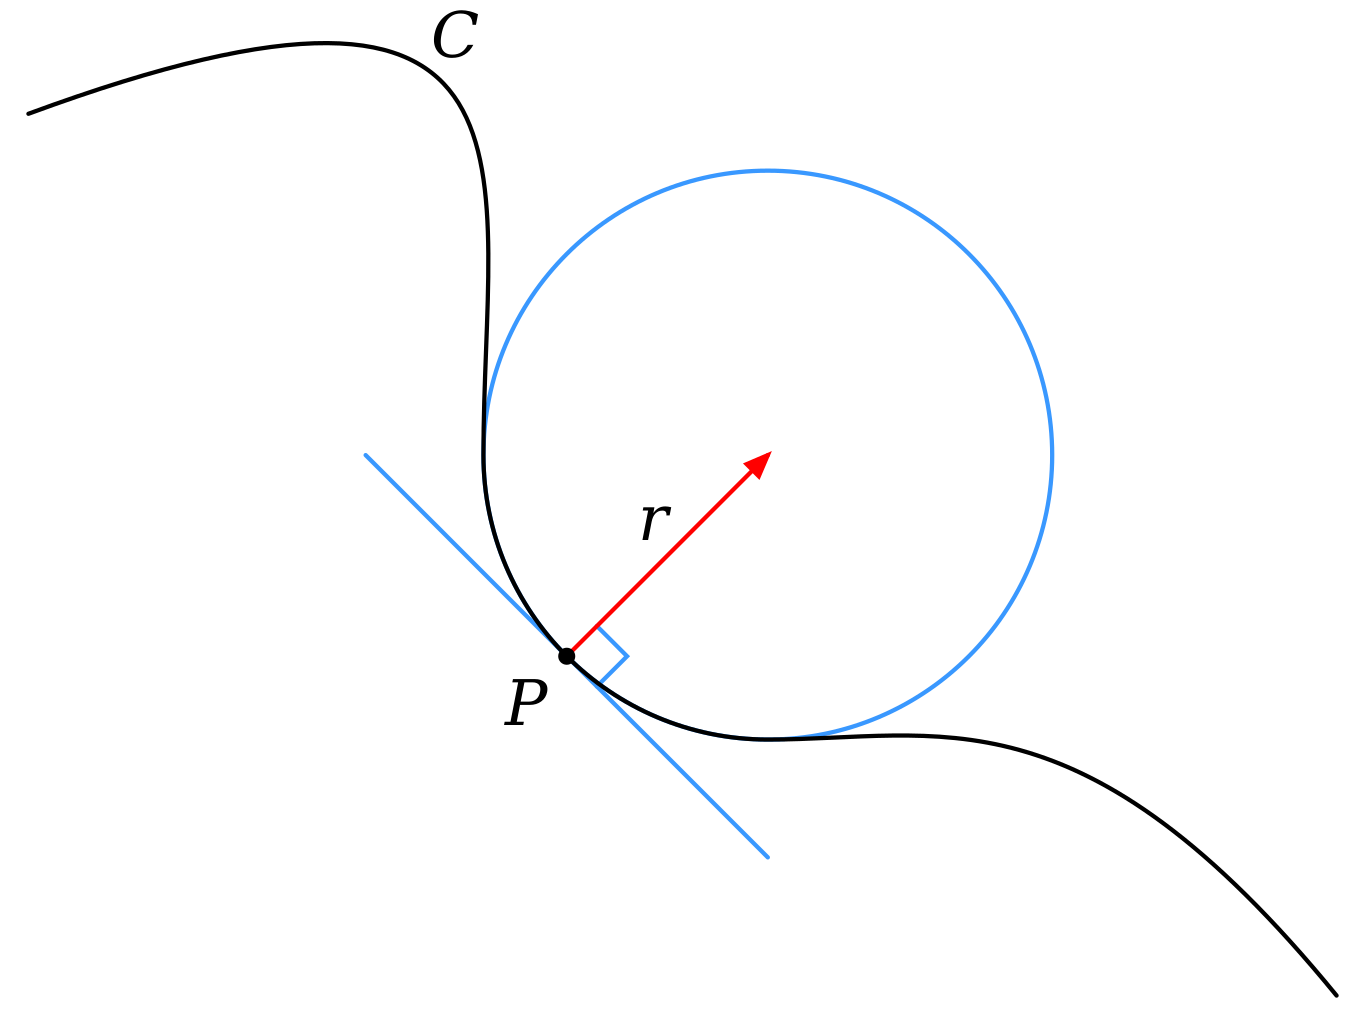
\includegraphics[scale=0.1]{minimal/Kruemmungsradius.png}
  \caption{Krümmungsradius} 
  \label{Kruemmungsradius}
\end{figure}

%Überträgt man das Konzept der Krümmung ins Dreidimensionale braucht es zwei Krümmungen, welche orthogonal zueinander stehen, um die Krümmung an einem Punkt zu bestimmen. Diese werden als Hauptkrümmungen $k_1$ und $k_2$ bezeichnet.
%Zur nummerischen Charakterisierung der Krümmung einer Fläche in der Mathematik werden hauptsächlich zwei Grössen benutzt.
%Zum einen die Gauss Krümmung, welche eine intrinsische Krümmung ist und zum andern die mittlere Krümmung bei welcher es sich um eine extrinsische Krümmung handelt. Bei Minimalflächen ist vor allem die mittlere Krümmung von Bedeutung.




\index{Gausskrümmung}
\subsubsection{Gauss Krümmung}
%Die Gauss Krümmung einer Fläche im Punkt $P$ ist definiert als das Produkt der zwei Hauptkrümmungen %$k_1$ und $k_2$.
%
%\begin{equation} \label{Gauss_Kruemmung_D}
%  K=k_1\, k_2= \frac{1}{R_1}\frac{1}{R_2}
%\end{equation}
%
%Die Gauss Krümmung ist eine intrinsische Krümmung. Ein Mass für die innere Krümmung der Fläche. 
%
In den vorhergehenden Kapiteln wurde hauptsächlich die Gausskrümmung betrachtet.
Dies weil wir uns auf der Erde in (oder direkt auf) der zu betrachtenden Fläche befinden und die gestellten Probleme innerhalb der Fläche eingebettet sind.   

Eine gute Vorstellungshilfe ist die Ameisenperspektive. 
Wenn eine Ameise auf einer Kugel ist kann sie feststellen, dass nur schon in ihrem kleinen Blickfeld die Winkelsumme eines Dreiecks auf der Oberfläche grösser als 180° ist, demzufolge besitzt die Kugel eine positive Gausskrümmung. Dies ist in der Abbildung \ref{skript:kruemmung:transportkugel} gut ersichtlich. Anders sieht es bei einem Zylinder aus. Dort misst die Ameise auf der Zylinderoberfläche genau 180° Winkelsumme, dass heisst die Gausskrümmung eines Zylinders ist null. Man kann sich dies leicht vorstellen, wenn man den Zylinder lediglich als aufgerollte Ebene ansieht. Zeichnet man beispielsweise ein Dreieck auf ein Blatt Papier, verändern sich die Winkel durch aufrollen des Papiers nicht. Im Gegensatz dazu verändern sich die Winkel auf einem Luftballon stark, wenn man diesen aufbläst. Dieser Effekt lässt sich gut in der Abbildung \ref{skript:kurven:4pifu2vis} sehen.

%Im Kontext dieses Buches ist noch zu erwähnen, dass für Flächen die Gausskrümmung genau dem Krümmungsskalar entspricht, dieses wurde im früheren Verlauf des Buches aus dem Riemann-Tensor abgeleitet (\ref{skript:maxima:curvature}).
Wie im Abschnitt \ref{skript:definition:gausskruemmung} Definition definiert wurde, ist die Gausskrümmung das Produkt der Hauptkrümmungen $k_1$ und $k_2$. 
Da wir intuitiv bei einem Kreis oder einer Kugel eine grosse Krümmungszahl erwarten und bei einer fast ebenen Fläche eine kleine, ist die Krümmung $k$ als der Kehrwert des Krümmungsradius $k=1/R$ definiert.
Wir schreiben damit die Gausskrümmung
\begin{equation} \label{Gauss_Kruemmung_D}
 K=k_1\, k_2= \frac{1}{R_1}\frac{1}{R_2}.
\end{equation}

\index{mittlere Krümmung}
\subsubsection{Mittlere Krümmung} 
%Die mittlere Krümmung einer Fläche im Punkt $P$ ist definiert durch den Mittelwert der zwei Hauptkrümmungen $k_1$ und $k_2$.

%\begin{equation} \label{Mittlere Kruemmung_D}
% H=\frac{1}{2}(k_1+k_2)= \frac{1}{2}\bigg(\frac{1}{R_1}+\frac{1}{R_2}\bigg)
%\end{equation}

Ebenfalls im Abschnitt 1.6.1 wurde bei Definition \ref{skript:definition:mittlerekruemmung2} die mittlere Krümmung definiert. Die mittlere Krümmung wird wie bei \eqref{Gauss_Kruemmung_D} zum besseren Verständnis zu
\begin{equation} \label{Mittlere Kruemmung_D}
H=\frac{1}{2}(k_1+k_2)= \frac{1}{2}\bigg(\frac{1}{R_1}+\frac{1}{R_2}\bigg)
\end{equation}
umgeschrieben.
Im Gegensatz zur intrinsischen Gausskrümmung, kommt es bei der extrinsischen mittleren Krümmung auf die Umgebung an. Beziehungsweise wie die Fläche in der Umgebung eingebettet ist.
Man stellt sich wieder die Mantelfläche eines Zylinders im dreidimensionalen Raum vor.
Aus der Ameisenperspektive ist die Mantelfläche eine zweidimensionale Fläche, betrachtet man die Mantelfläche jedoch von aussen, ist sie klar gekrümmt.
Dies, weil die Mantelfläche eine positive mittlere Krümmung aufweist. 
%dass man zum Beispiel die Krümmung eines Zylinders (zweidimensionales Objekt) von aussen, also in %einem dreidimensionalen Raum betrachtet. 
%Ein Zylinder ist aus der Ameisenperspektive flach, schaut man von aussen, sieht er jedoch gekrümmt %aus.


%Anders sieht es zum Beispiel bei einer Sattelfläche (Pringels-Chips artigen Fläche) aus, dort ist %die Gausskrümmung negativ, hingegen kann die mittlere Krümmung im Spezialfall, dass $R_1=-R_2$, %also die Krümmungsradien ein umgekehrtes Vorzeichen aufweisen, aber vom Betrag her identisch sind, %gleich null sein. 
Anders sieht es bei einer Sattelfläche aus (Abbildung \ref{fig:Scherk}). Hier ist die Gausskrümmung negativ. Daraus folgt, dass die Winkelsumme eines Dreiecks kleiner als 180° ist. Die mittlere Krümmung ist je nach Hauptkrümmungen $k_1$ und $k_2$ positiv oder negativ. In besonderen Fällen kann die mittlere Krümmung gleich null sein. Dies ist der Fall wenn die Hauptkrümmungen $k_1$ und $k_2$ vom Betrag gleich sind, aber umgekehrte Vorzeichen haben. Setzt man $k_2 = - k_1$ in die Gleichung \ref{Mittlere Kruemmung_D} ein,
\begin{equation}
H=\frac{1}{2}(k_1-k_1),
\end{equation}
erhält man 
\begin{equation}
H=\frac{1}{2}(0)=0.
\end{equation}

In diesem besonderen Fall ist die Sattelfläche ein Beispiel für eine Minimalfläche. Diese Eigenschaft führt auch dazu, dass jeder, genügend kleine Ausschnitt einer beliebigen Minimalfläche eine Sattelfläche ist. Nimmt man beispielsweise das Katenoid und halbiert es senkrecht erkennt man die vorhandene Sattelfläche (Abbildung \ref{fig:CatenoidHalf}). 

\begin{figure}
  \centering
  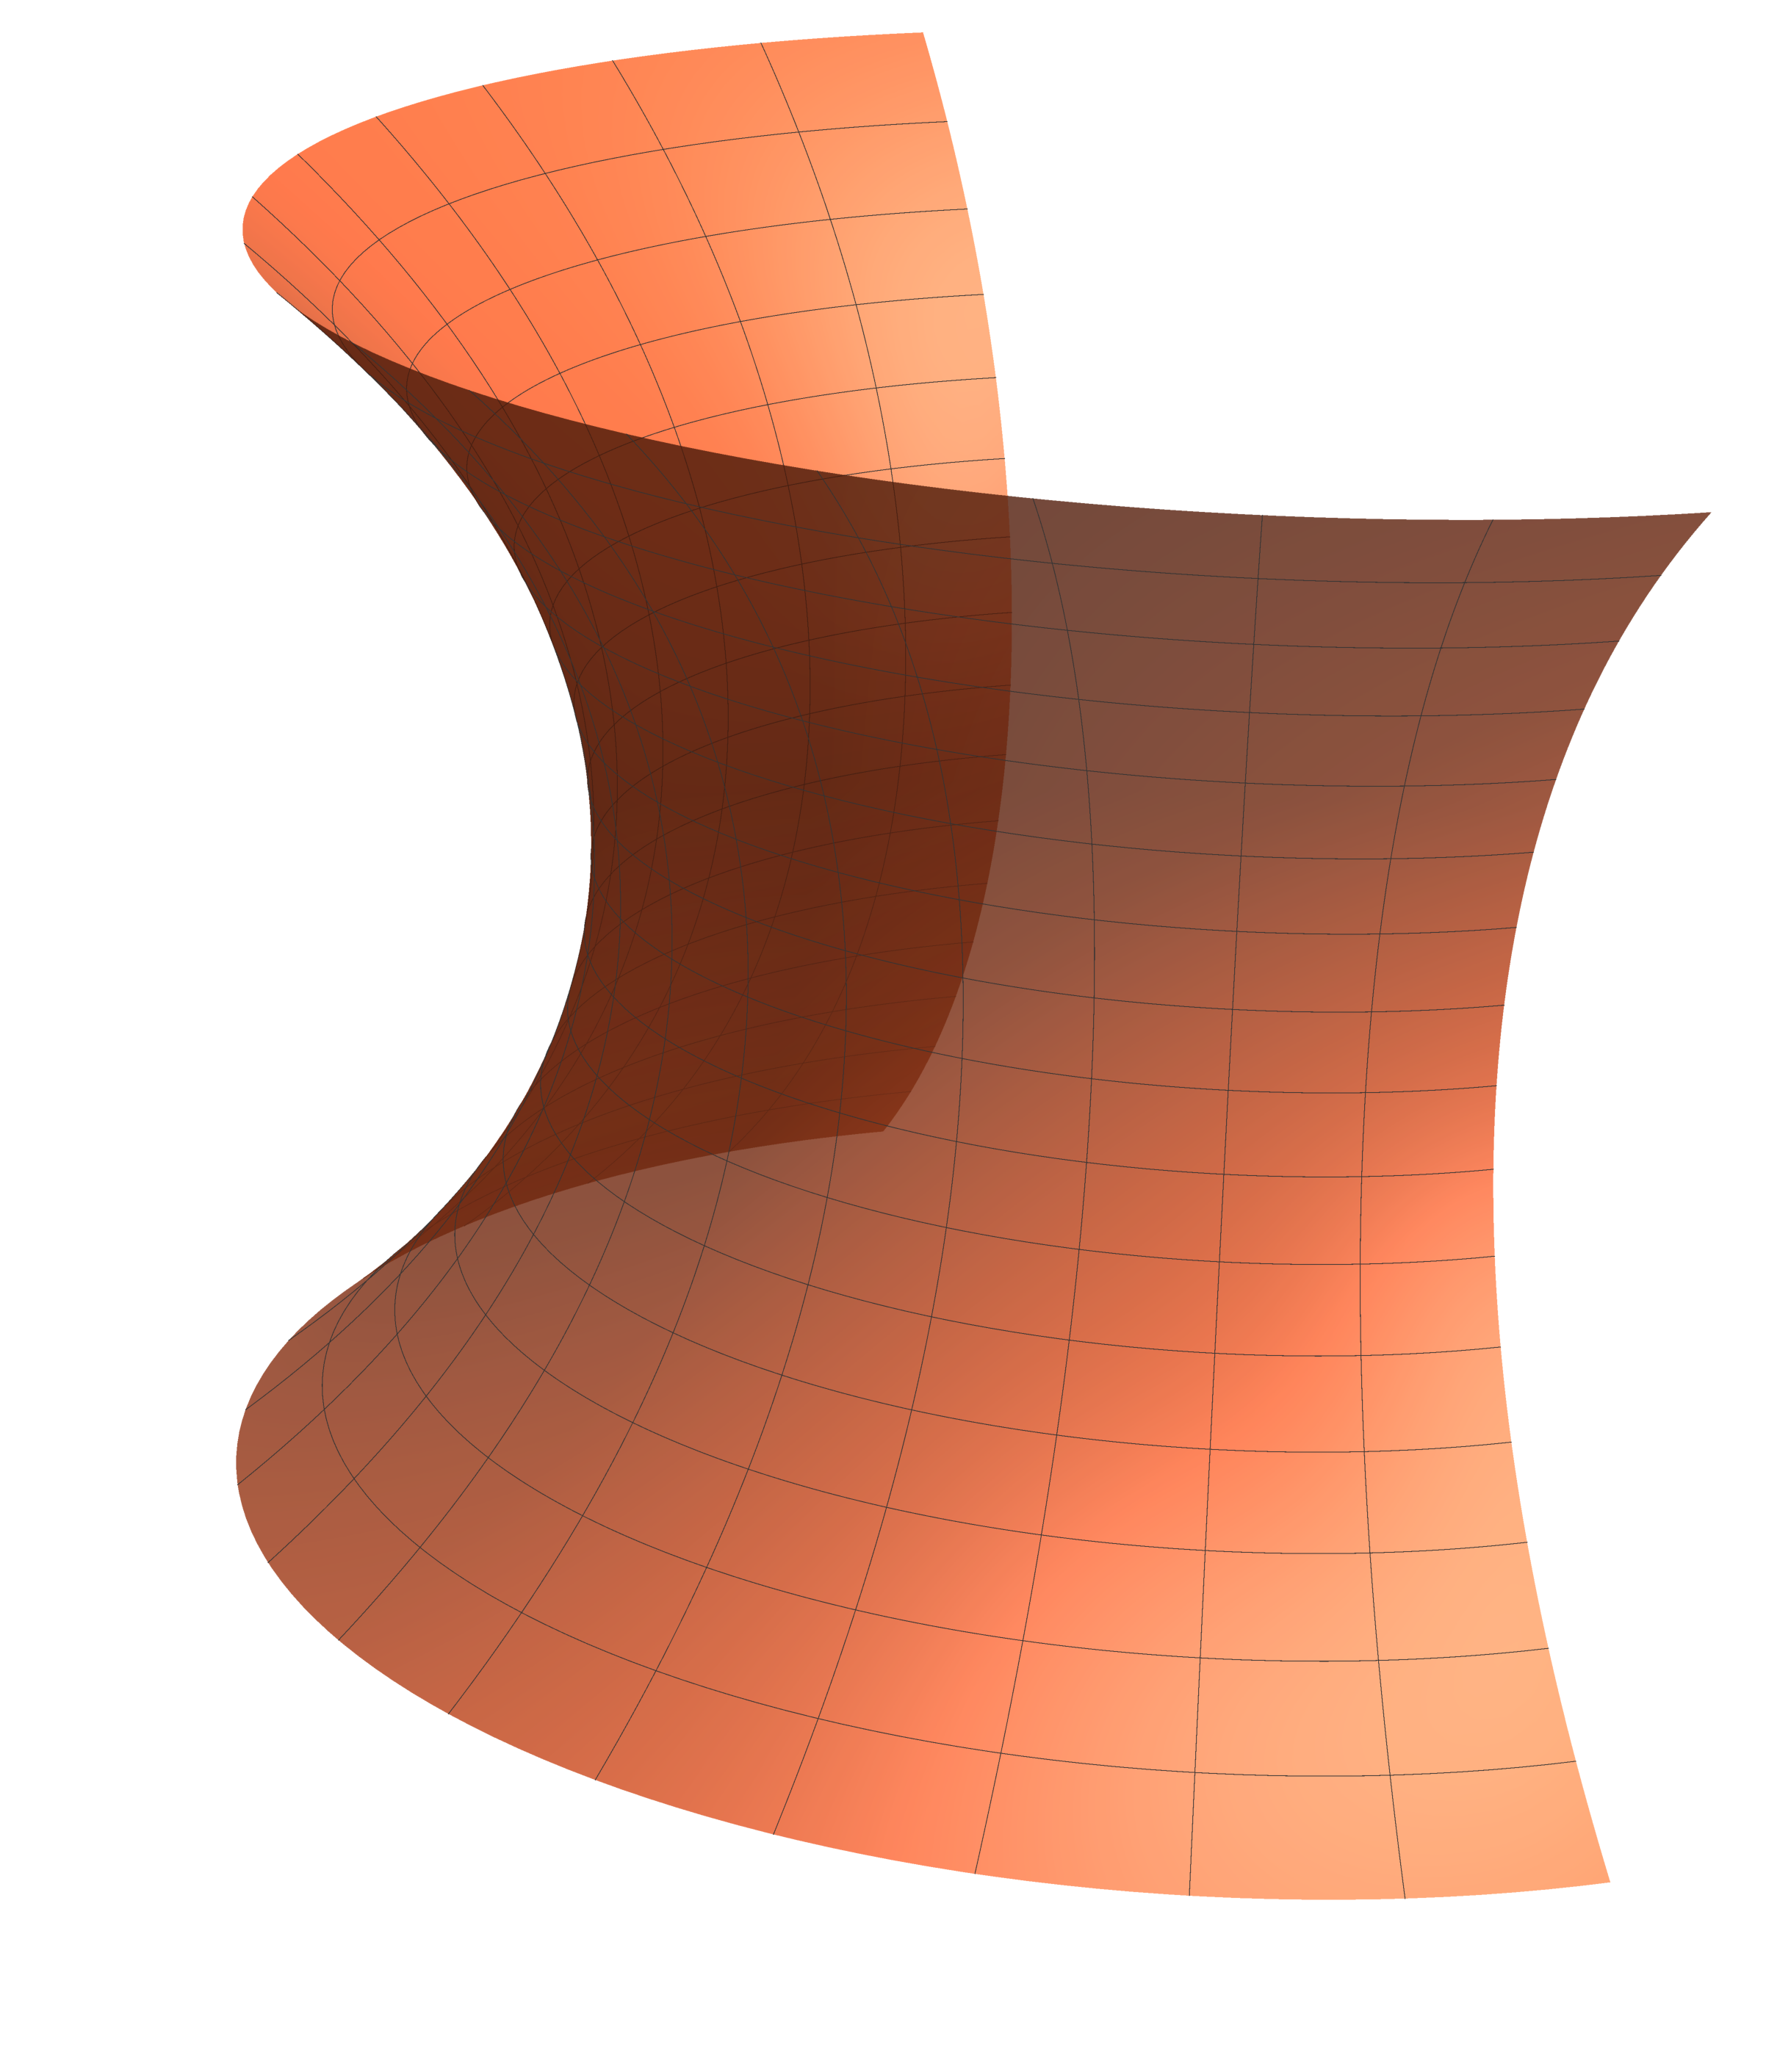
\includegraphics[angle=270,scale=0.1]{minimal/CatenoidHalf.pdf}
  \caption{Halbiertes Katenoid} 
  \label{fig:CatenoidHalf}
\end{figure}

\begin{figure} 
  \centering
  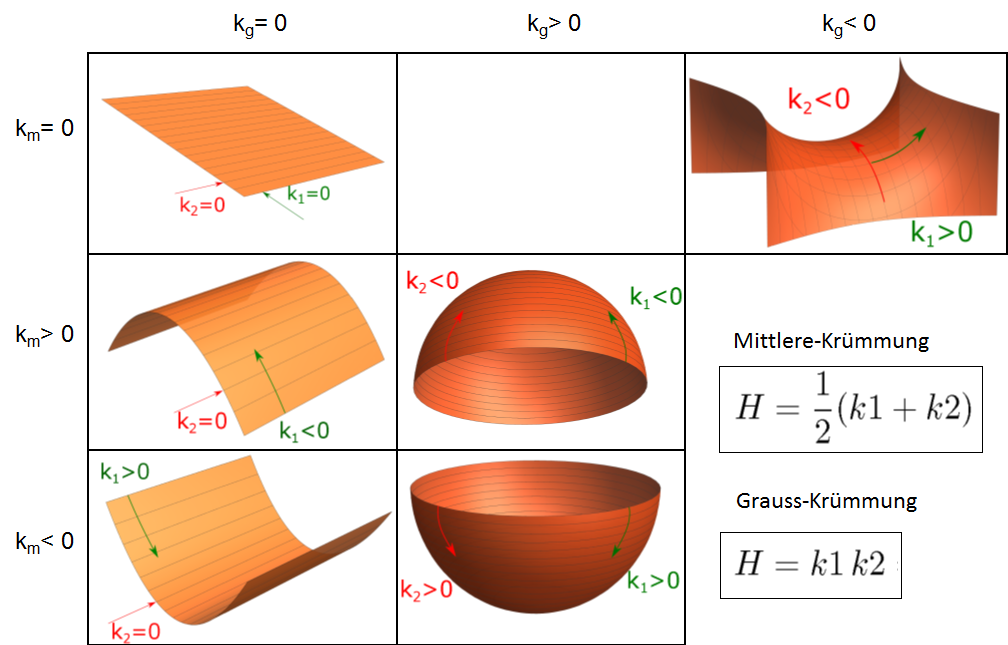
\includegraphics[scale=0.5]{minimal/Tabelle_Kruemmung.png}
  \caption{Vergleich Grausskrümmung und mittlere Krümmung} 
\end{figure}




\subsection{Beispiel Scherksche Sattelfläche}
\label{minimal:ScherkSattel}
\begin{figure}
  \centering
  \includegraphics[scale=0.3]{minimal/HFSherckV2.pdf}
  \caption{Sattelfläche von Scherk} 
  \label{fig:Scherk}
\end{figure}
Die Scherksche Sattelfläche wurde erstmals 1834 von H. F. Scherk beschrieben \cite{minimal:JournalAM}. Sie war nach der in 1776 von Meusnier beschriebene Katenoid die erste neue Minimalfläche. 

Die Scherksche Sattelfläche \, (Abbildung \ref{fig:Scherk})\, hat neben den zwingenden Eigenschaften einer Minimalfläche, deren Gausskrümmung kleiner als null ist und eine mittlere Krümmung von genau null hat. Die Eigenschaft, dass sie im Gegensatz zur Rotationsfläche des Katenoids, der Graph einer Funktion $z=Z(x,y)$ ist. 

Eine Approximation an die Fläche kann mittels Drahtgeflecht und einer Seifenlösung nachgebildet werden \, (Abbildung \ref{fig:SoapScherk}). Die einzelnen Seifenmoleküle versuchen ein stabiles Gleichgewicht der abstossenden und anziehenden Kräfte zu finden. Dieser stabile Punkt braucht durch das Gleichgewicht ein Minimum an Energie. Dies bedeutet auch, dass die Krümmung, welche Energie benötigt, minimiert wird.
\begin{figure}
  \centering
  \includegraphics[scale=0.4]{minimal/SattelflacheSoapFilm.png}
  \caption{Seifenfilm bildet Minimalfläche} 
  \label{fig:SoapScherk}
\end{figure}


Die mittlere Krümmung eines Graphen welcher mit $z=Z(x,y)$ definiert wird, kann auch mit $H=-\frac{1}{2} \nabla \cdot \hat{n}$\, \cite{minimal:Spivak}  berechnet werden, wobei $\hat{n}$ die normierte Normale auf der Ebene ist. Die Berechnung an sich ist recht aufwändig, deshalb wird hier nur das Ergebnis betrachtet:

\begin{equation}\label{MeanCurv}
H=\frac{Z_{xx}(Z_y^2+1) - 2 Z_xZ_yZ_{xy}+Z_{yy}(Z_x^2+1)}{\|\vec{n}\|^3}.
\end{equation}

Wobei ${x,y}$ die Koordinaten in der Ebene sind, welche nach $z$ abgebildet werden (siehe Abbildung \ref{fig:Scherk}). $Z_x$ ist die erste Ableitung der Funktion $Z(x,y)$ nach $x$. $Z_y$ ist analog dazu die erste Ableitung der Funktion $Z(x,y)$ nach $y$. $Z_{xx}$ und $Z_{yy}$ sind die jeweils zweite Ableitungen der Funktion $Z(x,y)$ nach den entsprechenden Indizes. $Z_{xy}$ ist die Ableitung von $Z_x$ nach $y$.

Wie wir im Kapitel \ref{Young-Laplace} sehen werden, muss die mittlere Krümmung bei Minimalflächen gleich null sein. Damit können wir den Zähler der Gleichung \eqref{MeanCurv} gleich null setzen
\begin{equation}\label{MFG}
Z_{xx}(Z_y^2+1) - 2 Z_xZ_yZ_{xy}+Z_{yy}(Z_x^2+1)=0.
\end{equation}
Diese Gleichung ist als Minimalflächengleichung (im Englischen Minimal Surface Equation \cite{minimal:Osserman}) bekannt.

Mittels dieser partiellen Differentialgleichung kann die noch unbekannte Funktion $z=Z(x,y)$ berechnet werden. Was im folgenden Abschnitt auch getan wird.


\subsubsection{Lösen der partiellen Differentialgleichung}\label{Scherk Berechnung}
Angenommen $z=Z(x,y)$ ist der Graph einer Funktion. Um die Minimalflächengleichung zu lösen nehmen wir an, dass die Funktion $Z(x,y)$ eine lineare Zusammensetzung von zwei Funktionen ist. Die einfachste Möglichkeit dies zu erreichen, ist die Addition von zwei Funktionen: $z=Z(x,y)=f(x)+g(y)$. Dieser Separationsansatz ist nur eine von vielen Möglichkeit eine partielle Differentialgleichung zu lösen.

Zusätzlich stellen wir zwei Nebenbedingungen. Die erste Bedingung, $Z(0,0)=0$, bedingt, dass der Graph im Nullpunkt auf der Höhe null ist. Die Zweite, $\nabla Z(0,0)=0$, fordert, dass im Nullpunkt der Graph horizontal ist.

Wir setzen die benötigten Ableitungen und mehrfachen Ableitungen der Funktion $Z(x,y)$ in die Minimalflächengleichung (\ref{MFG}) ein. Da $ Z_x = f'(x),\ Z_y = g'(y),\ Z_{xx}=f''(x),\ Z_{yy} = g''(y) \ \text{und} \ Z_{xy}=0$ ist, vereinfacht sich die Minimalflächengleichung zu 
\begin{equation}\label{MFG Scherk}
(1+g'(y)^2)f''(x)+(1+f'(x)^2)g''(y)=0
\end{equation}
Durch Separieren von $f$ und $g$ erhalten wir zwei gewöhnliche Differentialgleichungen zweiter Ordnung
\begin{equation}\label{MFG Scherk2}
-\dfrac{f''(x)}{1+(f'(x))^2}=\dfrac{g''(y)}{1+(g'(y))^2}=c
\end{equation}
mit $c \in \mathbb{R}$ konstant. $c$ ist konstant, da die Gleichung nur stimmen kann, wenn trotz unterschiedlichen Variablen $x$ und $y$ beide Quotienten bei einer Veränderung in $x$- beziehungsweise $y$-Richtung gleich bleiben. Wird zum Beispiel $x=0$ fixiert und $y$ variiert, muss die Differentialgleichung in $g(y)$ konstant bleiben, da sonst die Gleichung durch die Veränderung des zweiten Quotienten ungleich wäre. Ist $c=0$ tritt der spezielle Fall der Ebene ein. Diese ist vielfach, zum Beispiel bei einem einfachen Kreisring, auch intuitiv die Lösung einer Minimalfläche.

Die Differentialgleichungen in $f$ und $g$ werden nun separat gelöst. Erst wird $f'(x)$ mit $w(x)$ substituiert. 
\begin{equation}\label{ScherkDGL1}
-\dfrac{w'(x)}{1+w(x)^2}= c  , \quad w(x)=f'(x).
\end{equation}
Anschliessend wird die Gleichung  beidseitig integriert
\begin{equation}
\int -\dfrac{w'(x)}{1+w(x)^2} dx = \int c \ dx
\end{equation}
und wir erhalten die folgende Gleichung:
\begin{equation}
-\arctan(w(x)) = cx+k_1,
\end{equation}
welche wir nach $w(x)$ auflösen:
\begin{equation}
w(x) = -\tan(cx+k_1).
\end{equation}
Wir führen eine Rücksubstitution durch und erhalten
\begin{equation}\label{SchreckDGL2}
f'(x) = -\tan(cx+k_1).
\end{equation}
Um die Lösung der Differentialgleichung zu erhalten integrieren wir erneut
\begin{equation}
\int f'(x)\ dx = \int -\tan(cx+k_1)\ dx.
\end{equation}
 Die Lösung lautet
\begin{equation}
f(x) = \dfrac{\log(\cos(cx+k_1))}{c}+k_2.
\end{equation}
Mit den Nebenbedingung $f(0)=0$ und $f'(0)=0$ ergibt sich $k_1=k_2=0$ und wir erhalten die gesuchte Gleichung 
\begin{equation}
f(x) = \dfrac{\log(\cos(cx))}{c}.
\end{equation}
Analog dazu ergibt sich für die zweite Differentialgleichung:
\begin{equation}
g(y) = - \dfrac{\log(\cos(cx))}{c}.
\end{equation}
Somit lautet die Funktion $Z(x,y)$ der Scherkschen Minimalfläche
\begin{equation}
Z(x,y)=\dfrac{\log(\cos(cx))}{c}-\dfrac{\log(\cos(cy))}{c}.
\end{equation}

\subsection{Beispiel Young–Laplace - Oberflächenspannung}
\rhead{Young–Laplace}
\label{Young-Laplace}

\label{YL-Beschreibung}
In den vorangegangenen Beispielen wurde jeweils eine Lösung gesucht, bei der die mittlere Krümmung $H=0$ ist. Bei den meisten Oberflächen ist dies jedoch nicht der Fall. Beispielsweise haben Seifenblasen innen und aussen einen anderen Druck. Oder in einem Blutgefäss herrscht innen der Blutdruck und außerhalb der Druck durch das Gewebe. Diese Druckdifferenz wirkt eine Kraft auf eine Oberfläche ein und verunmöglicht damit eine minimale Oberfläche wie bei einer Minimalfläche.

Dennoch haben solche Oberflächen ähnliche Eigenschaften, da auch hier die Energie minimiert wird. Dies wird durch die Young-Laplace Gleichung \cite{minimal:Laplace} beschrieben, welche im folgenden Abschnitt mittels geometrischen und physikalischen Überlegungen hergeleitet wird.

\subsubsection{Herleitung der Young-Laplace Gleichung}\label{YL-Herleitung}
Angenommen zwei Medien (z.B. Luft/Wasser) werden durch eine Oberfläche \, (Abbildung \ref{fig:YoungCone}) getrennt. Da in den Medien verschiedene Drücke $p_1$ und $p_2$ herrschen, wölbt sich die Oberfläche. Die Veränderung des Krümmungsradius sei $\delta\zeta$ \,(Abbildung \ref{fig:Strahlensatz}). Das Volumen eines einzelnen infinitesimalen Volumensegments sei $\delta\zeta\,dA$ \,(Abbildung \ref{fig:Volumentransaltion}). Dann ist die benötigte Arbeit um das Volumensegment um $\delta\zeta$ zu verschieben:
\begin{figure}
  \centering
  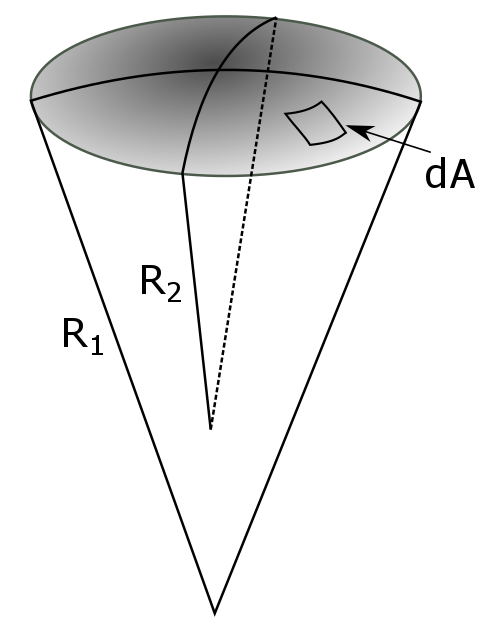
\includegraphics[scale=0.3]{minimal/YoungCone.png}
  \caption{Ausschnitt aus einer Oberfläche mit Krümmungsradien} 
  \label{fig:YoungCone}
\end{figure}
\begin{figure}
  \centering
  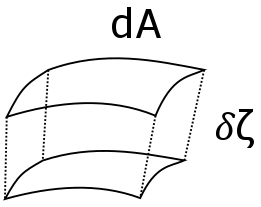
\includegraphics[scale=0.3]{minimal/Volumetranslation.png}
  \caption{Element der Volumentranslation} 
  \label{fig:Volumentransaltion}
\end{figure}
\begin{equation}
\delta W=\int(-p_1+p_2)\,\delta\zeta\,dA.
\end{equation}
Die gesamte Arbeit ergibt sich, wenn zur Arbeit der Volumenänderung die Arbeit der Veränderung der Oberfläche $\delta W=\gamma \, \delta A $ dazu addiert wird, wobei $\gamma$ die Oberflächenspannung und $\delta A$ die veränderte Oberfläche ist. Wir erhalten
\begin{equation}\label{YL-Arbeit_1}
\delta W=\int(-p_1+p_2)\,\delta\zeta dA + \gamma \,\delta A.
\end{equation}
Sind $R_1$ und $R_2$ die Krümmungsradien der Oberfläche, werden die infinitesimalen Längenstücke $dl_1$ und $dl_2$ bei einer Veränderung der Radien $R$ um $\delta\zeta$ mittels Strahlensatz \,(Abbildung \ref{fig:Strahlensatz})
\begin{equation}
\frac{R}{dl}=\frac{R+\delta\zeta}{dl+x}
\end{equation}
verlängert. Wobei $dl+x=dl'$ ist. Nach $dl'$ aufgelöst ergibt sich
\begin{equation}
dl' = dl\bigg(\frac{R+\delta\zeta}{R}\bigg)
\end{equation}
durch einfache Umformungen erhalten wir
\begin{equation}
\begin{split}
dl' &= dl\bigg(1+\frac{\delta\zeta}{R}\bigg)\\
&=dl+\frac{dl\,\delta\zeta}{R} .
\end{split} 
\end{equation}
\begin{figure}
  \centering
  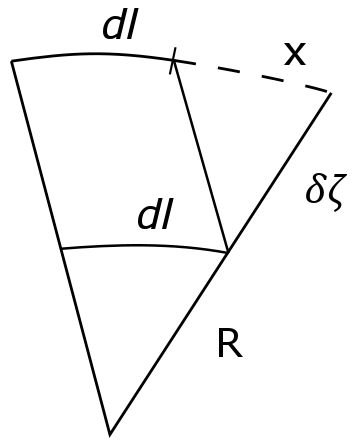
\includegraphics[scale=0.3]{minimal/Langenanderung2.png}
  \caption{Längenänderung} 
  \label{fig:Strahlensatz}
\end{figure}
Das Flächenstück $dA=dl_1 dl_2$ verändert sich somit
\begin{equation}
\begin{split}
dA' &= \bigg(1+\frac{\delta\zeta}{R_1}\bigg)\, dl_1 \bigg(1+\frac{\delta\zeta}{R_2}\bigg) \, dl_2 \\
&\approx dl_1\,dl_2\,\bigg(1+\frac{\delta\zeta}{R_1} + \frac{\delta\zeta}{R_2}\bigg).
\end{split}
\end{equation} 
Somit ist die Änderung eines Flächenstück $\delta dA=dA'-dA$
\begin{equation}
\begin{split}
\delta dA &= dl_1\,dl_2\,\delta\zeta\,(1+\frac{1}{R_1}+\frac{1}{R_2})-dl_1\,dl_2\\
&= dl_1\,dl_2\,\delta\zeta\,(\frac{1}{R_1}+\frac{1}{R_2}).
\end{split}
\end{equation}
Um die gesamte veränderte Oberfläche zu erhalten, integrieren wir die Änderung der Flächenstücke über die gesamte Oberfläche
\begin{equation}
\delta A = \int \delta\zeta \, \bigg( \frac{1}{R_1}+\frac{1}{R_2} \bigg)\,dA.
\end{equation}
Die veränderte Oberfläche setzen wir in die Gleichung der Variation der Arbeit \ref{YL-Arbeit_1} ein. 
Befindet sich die Oberfläche im Gleichgewicht, muss auch die Variation der Arbeit gleich Null sein:
\begin{equation} \label{YL-Rechnung7}
\delta W = \int \delta\zeta \, \bigg[ (-p_1+p_2)-\gamma \, \bigg( \frac{1}{R_1}+\frac{1}{R_2} \bigg) \bigg]\,dA =0.
\end{equation}
Da $\delta\zeta=0$ eine triviale Lösung wäre, ist $\delta\zeta \neq 0$. Darum muss die eckige Klammer aus der vorherigen Gleichung gleich null sein. Daraus folgt die Young-Laplace Gleichung:
\begin{equation}
-p_1+p_2 = \gamma \, \bigg( \frac{1}{R_1}+\frac{1}{R_2} \bigg)
\end{equation}
oder
\begin{equation}\label{Young-Laplace-Equation}
\Delta p = \gamma \, \bigg( \frac{1}{R_1}+\frac{1}{R_2} \bigg).
\end{equation}
Anzumerken ist, dass sie der Gleichung der mittleren Krümmung (\ref{Mittlere Kruemmung_D}) bis auf $2\gamma$ entspricht. Wir lösen die Gleichung der mittleren Krümmung nach $( \frac{1}{R_1}+\frac{1}{R_2} )$ auf und erhalten
\begin{equation}
\bigg( \frac{1}{R_1}+\frac{1}{R_2} \bigg)=2H.
\end{equation}
Somit kann man die Young-Laplace Gleichung auch als
\begin{equation}\label{YL-Result2}
\Delta p=2\gamma H
\end{equation}
schreiben.

\subsubsection{Schlussfolgerung}\label{YL-conclusion}
Ist der Druckunterschied $\Delta p =0$, was beispielsweise bei einem Seifenfilm der Fall ist, muss entweder $\gamma$ oder $H$ gleich null sein. Da im allgemeinen Fall  die Oberflächenspannung $\gamma$ ungleich null ist \cite{minimal:Eotvos},  schliessen wir daraus, dass bei  $\Delta p =0$ die mittlere Krümmung gleich null sein muss.

\subsection{Anwendung: Seifenblase}
Durch die in der Schlussfolgerung gewonnene Erkenntnis ist klar, dass eine Seifenblase keine Minimalfläche sein kann, da zwischen der Luft innen und aussen der Seifenblase immer ein Druckunterschied vorhanden ist.

\subsection{Anwendung: Druck innerhalb eines Regentropfens}
Nehmen wir an, ein Regentropfen wird nicht durch den Luftwiderstand verformt, so bildet er eine Kugel. Da bei einer Kugel $R_1=R_2=r$ gilt, vereinfacht sich die Young-Laplace Gleichung \ref{Young-Laplace-Equation} zu
\begin{equation}
\Delta p = 2\gamma \, \bigg(\frac{1}{r}\bigg).
\end{equation}
Bei einem Radius von $0.2\text{mm}$ und einer Oberflächenspannung von $72.75 \text{mN}/\text{m}$ erhalten wir eine Druckdifferenz von
\begin{equation}
\Delta p = 2 \cdot 72.75 \text{mN}/\text{m} \, \bigg(\frac{1}{0.2\text{mm}}\bigg)= 727.5 \text{Pa},
\end{equation}
was in der Grössenordnung von einem Hundertstel des atmosphärischen Drucks liegt. 

%\subsection{Anwendung: Seifenblasen sind keine Minimalfläche}
%Mithilfe der bei \ref{YL-Result2} gewonnen Erkenntnis können wir leicht erkennen, dass bei einem %Druckunterschied auf beiden Seiten eines Seifenfilms, Beispielsweise bei einer Seifenblase, die %mittlere Krümmung nicht null sein kann. Somit kann eine Seifenblase nicht eine Minimalfläche sein.

\iffalse
\subsubsection{Minimalflächengleichung}\label{MFG}
\begin{equation}
\begin{split}
\vec{n} &= \begin{pmatrix}Z_x \\ Z_y \\ -1\end{pmatrix} \\
\|\vec{n}\| &= \sqrt{Z_x^2+Z_y^2+1} \\
\hat{n} &= \frac{\vec{n}}{\|\vec{n}\|} \\
\end{split}
\end{equation}

\begin{equation}
\nabla \cdot \hat{n} = \frac{\partial}{\partial x} \frac{Z_x}{\|\vec{n}\|} + \frac{\partial}{\partial y} \frac{Z_y}{\|\vec{n}\|} + \frac{\partial}{\partial z}\frac{-1}{\|\vec{n}\|}
\end{equation}
\begin{equation}
\frac{\partial}{\partial x} \frac{Z_x}{\|\vec{n}\|} = \frac{1}{\|\vec{n}\|} \frac{\partial Z_x}{\partial x} + Z_x \frac{\partial}{\partial x} \frac{1}{\|\vec{n}\|}
\end{equation}
\begin{equation}
\frac{\partial}{\partial x} \frac{1}{\|\vec{n}\|} = \frac{\partial}{\partial x} (Z_x^2+Z_y^2+1)^{-1/2} = \frac{-\frac{1}{2} (2\frac{\partial Z_x}{\partial x} + 2\frac{\partial Z_y}{\partial x})}{\|\vec{n}\|^3} =\frac{-(Z_x Z_{xx}+Z_y Z_{xy})}{\|\vec{n}\|^3}
\end{equation}
\begin{equation}
\frac{\partial}{\partial x} \frac{Z_x}{\|\vec{n}\|} = \frac{Z_{xx}}{\|\vec{n}\|}-\frac{Z_x(Z_x Z_{xx} + Z_y Z_{xy})}{\|\vec{n}\|^3}
\end{equation}
Äquivaltnt für d/dy
\begin{equation}
\frac{\partial}{\partial z}\frac{-1}{\|\vec{n}\|}=0
\end{equation}
\begin{equation}
\begin{split}
\nabla \cdot \hat{n} &= \frac{Z_{xx}}{\|\vec{n}\|}-\frac{Z_x(Z_x Z_{xx} + Z_y Z_{xy})}{\|\vec{n}\|^3} + \frac{Z_{yy}}{\|\vec{n}\|}-\frac{Z_y(Z_y Z_{yy} + Z_x Z_{xy})}{\|\vec{n}\|^3} \\
&=\frac{Z_{xx}\|\vec{n}\|^2 - Z_x(Z_x Z_{xx} + Z_y Z_{xy}) + Z_{yy}\|\vec{n}\|^2 - Z_y(Z_y Z_{yy} + Z_x Z_{xy})}{\|\vec{n}\|^3}
\end{split}
\end{equation}
\begin{equation}
\begin{split}
\nabla \cdot \hat{n} &= \frac{Z_{yy}(Z_x^2+Z_y^2+1)-Z_x^2Z_{xx} - Z_xZ_yZ_{xy}}{\|\vec{n}\|^3} \\
& \quad \frac{+ \, Zyy(Z_x^2+Z_y^2+1)-2_y^2Z_{yy}-Z_yZ_xZ_{xy}}{\|\vec{n}\|^3} \\
&= \frac{Z_{yy}(Z_y^2+1) - 2 Z_xZ_yZ_{xy}+Zyy(Z_x^2+1)}{\|\vec{n}\|^3}
\end{split}
\end{equation}
\fi


\printbibliography[heading=subbibliography]
\end{refsection}
